\begin{frame}{LoRA and Quantized LoRA}
  \begin{center}
    \Large
    LoRA and Quantized LoRA
  \end{center}
\end{frame}

\begin{frame}[t]{What is LoRA?}
  \begin{itemize}\itemsep0.4em
    \item[\textcolor{red}{$\blacktriangleright$}] \textbf{Key Idea:} Freeze the pre-trained weights and learn a low-rank update instead.
    \item[\textcolor{red}{$\blacktriangleright$}] For a weight matrix $W \in \mathbb{R}^{d \times k}$:
      \[
      W' = W + \tfrac{\alpha}{r}\,\Delta W, \quad \Delta W = BA
      \]
      with $B \in \mathbb{R}^{d \times r}$, $A \in \mathbb{R}^{r \times k}$, and rank $r \ll \min(d,k)$.
    \item[\textcolor{red}{$\blacktriangleright$}] Only $A$ and $B$ are trained: $r(d+k)$ parameters in place of $dk$.
    \item[\textcolor{red}{$\blacktriangleright$}] $A$ is initialised from a Gaussian and $B$ to zero, so $\Delta W = 0$ at the first step and training starts from exactly the pre-trained model.
    \item[\textcolor{red}{$\blacktriangleright$}] The scale $\alpha/r$ keeps the size of the update roughly independent of $r$, so changing the rank does not force a learning-rate retune.
  \end{itemize}
\end{frame}

\begin{frame}{What is LoRA?}
  \begin{figure}
    \centering
    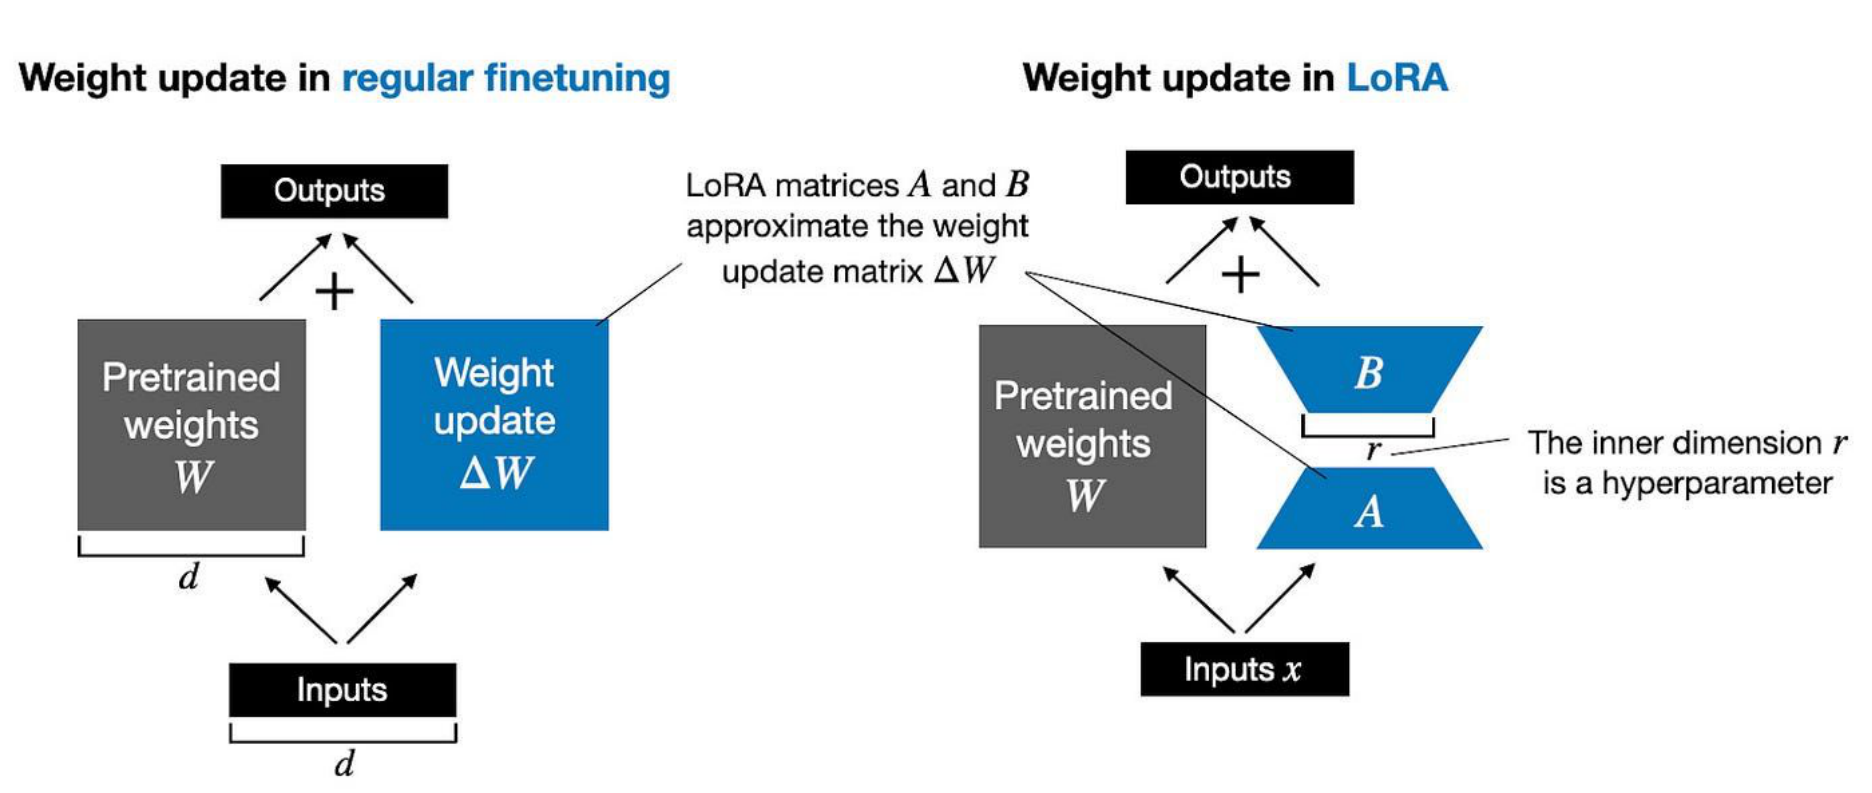
\includegraphics[width=0.80\paperwidth,height=0.60\paperheight,keepaspectratio]{images/llm-rlhf/finetune_lora_weight_update.png}
    \caption*{\scriptsize Sebastian Raschka, ``Practical Tips for Finetuning LLMs Using LoRA (Low-Rank Adaptation),'' \textit{Ahead of AI}, 2023.}
  \end{figure}
\end{frame}

\begin{frame}[t]{Benefits of LoRA}
  \begin{itemize}\itemsep0.4em
    \item[\textcolor{red}{$\blacktriangleright$}] \textbf{Very lightweight:} Well under 1\% of parameters are trainable, and the fraction shrinks as the base model grows: about 0.2\% for RoBERTa-large, and as little as 0.01\% for GPT-3 175B, a $10{,}000\times$ cut (Hu et al., 2021).
    \item[\textcolor{red}{$\blacktriangleright$}] \textbf{Hardware friendly:} Enables fine-tuning on consumer GPUs and even laptops.
    \item[\textcolor{red}{$\blacktriangleright$}] \textbf{No inference overhead:} $BA$ can be folded back into $W$ once training ends, so a deployed LoRA model runs at exactly the speed of the base model.
    \item[\textcolor{red}{$\blacktriangleright$}] \textbf{Modular:} Supports plug-and-play adapters for different tasks or users.
    \item[\textcolor{red}{$\blacktriangleright$}] \textbf{Personalization:} Allows efficient user- or domain-specific adaptation.
  \end{itemize}
\end{frame}

\begin{frame}{QLoRA --- Quantized LoRA}
  \begin{itemize}
    \item[\textcolor{red}{$\blacktriangleright$}] \textbf{Key Idea:} Fine-tune large language models in 4-bit precision using LoRA adapters.
    \item[\textcolor{red}{$\blacktriangleright$}] \textbf{Scalability:} Enables fine-tuning of 65B parameter models on a single 48GB GPU.
    \item[\textcolor{red}{$\blacktriangleright$}] \textbf{Efficiency:} Matches full 16-bit fine-tuning on the benchmarks tested; the authors note that parity at 33B and 65B was not established (Dettmers et al., 2023).
    \item[\textcolor{red}{$\blacktriangleright$}] \textbf{Techniques:}
      \begin{itemize}
        \item 4-bit NormalFloat (NF4), a storage type matched to normally distributed weights
        \item Double quantization: quantize the quantization constants too
        \item Paged optimizers, to absorb memory spikes
      \end{itemize}
    \item[\textcolor{red}{$\blacktriangleright$}] Weights are \emph{stored} in 4 bits but dequantized to BFloat16 for each matrix multiply, so compute precision is unchanged.
  \end{itemize}
\end{frame}

\begin{frame}{QLoRA --- Quantized LoRA}
  \begin{figure}
    \centering
    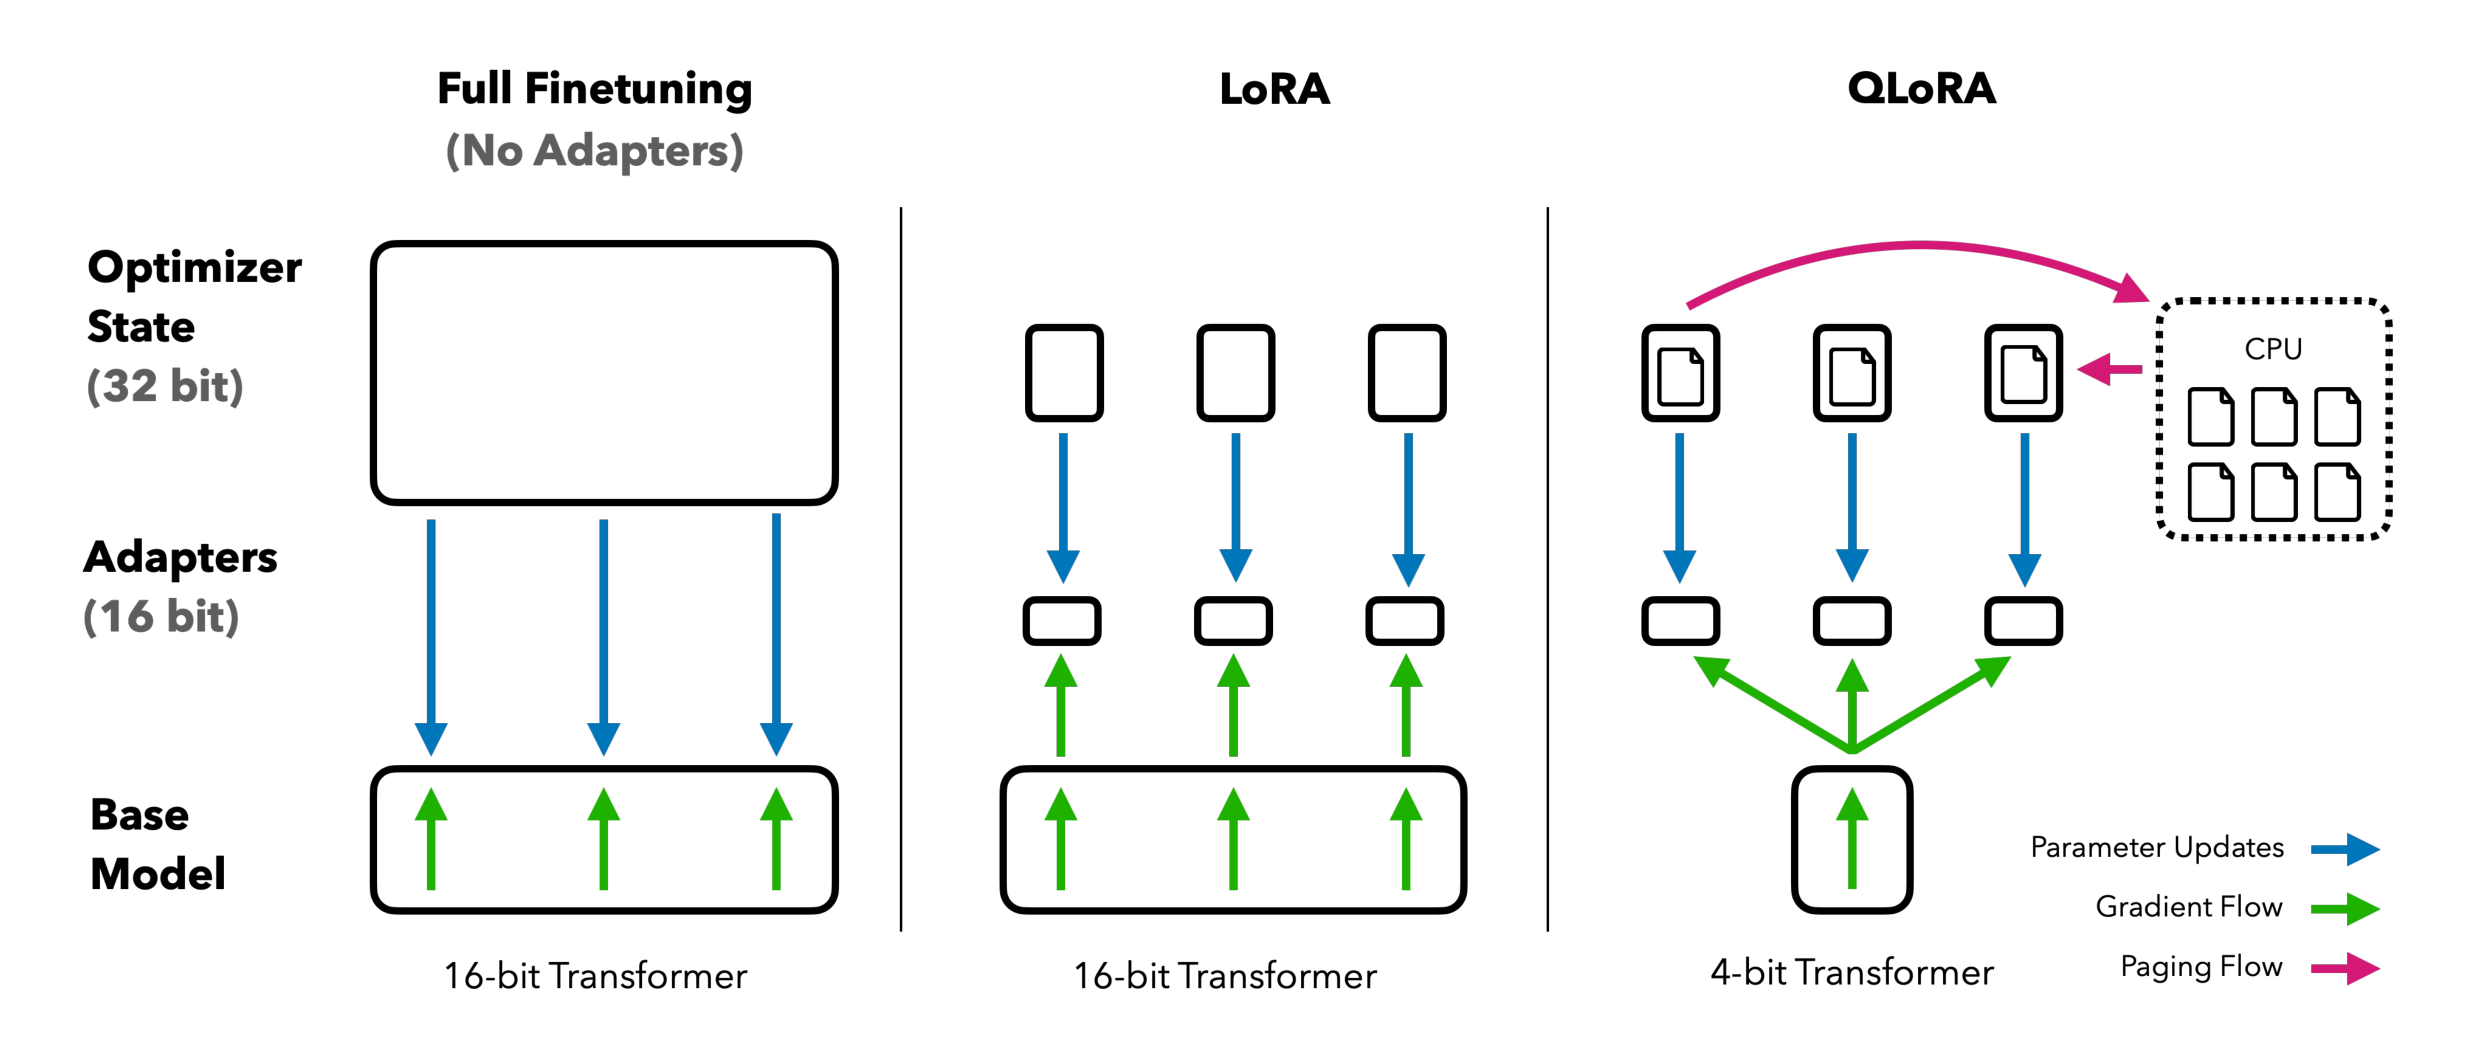
\includegraphics[width=0.88\paperwidth,height=0.58\paperheight,keepaspectratio]{images/llm-rlhf/qlora_memory_footprint_fig1.png}
    \caption*{\scriptsize Dettmers, Pagnoni, Holtzman \& Zettlemoyer, ``QLoRA: Efficient Finetuning of Quantized LLMs,'' NeurIPS 2023, Fig.~1.}
  \end{figure}
\end{frame}

\begin{frame}{Applications of LoRA / QLoRA}
  \begin{itemize}
    \item[\textcolor{red}{$\blacktriangleright$}] \textbf{Instruction tuning for resource-constrained settings:}
      \begin{itemize}
        \item Enables fine-tuning large models on modest hardware (e.g., consumer GPUs, laptops).
        \item Used for domain adaptation, personalization, and rapid prototyping.
      \end{itemize}
    \item[\textcolor{red}{$\blacktriangleright$}] \textbf{Models tuned this way:}
      \begin{itemize}
        \item \textbf{Guanaco} (Dettmers et al., 2023): a QLoRA fine-tune of LLaMA on OpenAssistant data; the 65B model trains in 24 hours on one 48GB GPU.
        \item Base models such as \textbf{LLaMA} and \textbf{Mistral} are the \emph{targets} of LoRA tuning, not products of it.
        \item The original \textbf{Alpaca} and \textbf{Vicuna} releases were full fine-tunes on 8$\times$A100; community LoRA reproductions came later.
      \end{itemize}
    \item[\textcolor{red}{$\blacktriangleright$}] \textbf{Model merging and compositionality:}
      \begin{itemize}
        \item Merge multiple LoRA adapters for multi-domain or multi-task capabilities.
        \item Compose adapters for new tasks without retraining the base model.
      \end{itemize}
  \end{itemize}
\end{frame}
